\chapter{优化算法}\label{ux7b2cux4e00ux5341ux4e09ux7ae0-ux4f18ux5316ux7b97ux6cd5}

\section{如何解决训练样本少的问题}\label{ux5982ux4f55ux89e3ux51b3ux8badux7ec3ux6837ux672cux5c11ux7684ux95eeux9898}

目前大部分的深度学习模型仍然需要海量的数据支持。例如 ImageNet
数据就拥有1400多万的图片。而现实生产环境中,数据集通常较小,只有几万甚至几百个样本。这时候,如何在这种情况下应用深度学习呢?\\
(1)利用预训练模型进行迁移微调(fine-tuning),预训练模型通常在特征上拥有很好的语义表达。此时,只需将模型在小数据集上进行微调就能取得不错的效果。这也是目前大部分小数据集常用的训练方式。视觉领域内,通常会ImageNet上训练完成的模型。自然语言处理领域,也有BERT模型等预训练模型可以使用。
   (2)单样本或者少样本学习(one-shot,few-shot
learning),这种方式适用于样本类别远远大于样本数量的情况等极端数据集。例如有1000个类别,每个类别只提供1-5个样本。少样本学习同样也需要借助预训练模型,但有别于微调的在于,微调通常仍然在学习不同类别的语义,而少样本学习通常需要学习样本之间的距离度量。例如孪生网络(Siamese
Neural
Networks)就是通过训练两个同种结构的网络来判别输入的两张图片是否属于同一类。
​
上述两种是常用训练小样本数据集的方式。此外,也有些常用的手段,例如数据集增强、正则或者半监督学习等方式来解决小样本数据集的训练问题。

\section{深度学习是否能胜任所有数据集?}\label{ux6df1ux5ea6ux5b66ux4e60ux662fux5426ux80fdux80dcux4efbux6240ux6709ux6570ux636eux96c6}

深度学习并不能胜任目前所有的数据环境,以下列举两种情况:

(1)深度学习能取得目前的成果,很大一部分原因依赖于海量的数据集以及高性能密集计算硬件。因此,当数据集过小时,需要考虑与传统机器学习相比,是否在性能和硬件资源效率更具有优势。
(2)深度学习目前在视觉,自然语言处理等领域都有取得不错的成果。这些领域最大的特点就是具有局部相关性。例如图像中,人的耳朵位于两侧,鼻子位于两眼之间,文本中单词组成句子。这些都是具有局部相关性的,一旦被打乱则会破坏语义或者有不同的语义。所以当数据不具备这种相关性的时候,深度学习就很难取得效果。

\section{有没有可能找到比已知算法更好的算法?}\label{ux6709ux6ca1ux6709ux53efux80fdux627eux5230ux6bd4ux5df2ux77e5ux7b97ux6cd5ux66f4ux597dux7684ux7b97ux6cd5}

在最优化理论发展中,有个没有免费午餐的定律,其主要含义在于,在不考虑具体背景和细节的情况下,任何算法和随机猜的效果期望是一样的。即,没有任何一种算法能优于其他一切算法,甚至不比随机猜好。深度学习作为机器学习领域的一个分支同样符合这个定律。所以,虽然目前深度学习取得了非常不错的成果,但是我们同样不能盲目崇拜。

优化算法本质上是在寻找和探索更符合数据集和问题的算法,这里数据集是算法的驱动力,而需要通过数据集解决的问题就是算法的核心,任何算法脱离了数据都会没有实际价值,任何算法的假设都不能脱离实际问题。因此,实际应用中,面对不同的场景和不同的问题,可以从多个角度针对问题进行分析,寻找更优的算法。

\section{什么是共线性,如何判断和解决共线性问题?}\label{ux4ec0ux4e48ux662fux5171ux7ebfux6027ux5982ux4f55ux5224ux65adux548cux89e3ux51b3ux5171ux7ebfux6027ux95eeux9898}

对于回归算法,无论是一般回归还是逻辑回归,在使用多个变量进行预测分析时,都可能存在多变量相关的情况,这就是多重共线性。共线性的存在,使得特征之间存在冗余,导致过拟合。

常用判断是否存在共线性的方法有:

(1)相关性分析。当相关性系数高于0.8,表明存在多重共线性;但相关系数低,并不能表示不存在多重共线性;

(2)方差膨胀因子VIF。当VIF大于5或10时,代表模型存在严重的共线性问题;

(3)条件系数检验。
当条件数大于100、1000时,代表模型存在严重的共线性问题。

通常可通过PCA降维、逐步回归法和LASSO回归等方法消除共线性。

\section{权值初始化方法有哪些?}\label{ux6743ux503cux521dux59cbux5316ux65b9ux6cd5ux6709ux54eaux4e9b}

在深度学习的模型中,从零开始训练时,权重的初始化有时候会对模型训练产生较大的影响。良好的初始化能让模型快速、有效的收敛,而糟糕的初始化会使得模型无法训练。

目前,大部分深度学习框架都提供了各类初始化方式,其中一般常用的会有如下几种:
\textbf{1. 常数初始化(constant)}

​
把权值或者偏置初始化为一个常数。例如设置为0,偏置初始化为0较为常见,权重很少会初始化为0。TensorFlow中也有zeros\_initializer、ones\_initializer等特殊常数初始化函数。

\textbf{2. 高斯初始化(gaussian)}

​
给定一组均值和标准差,随机初始化的参数会满足给定均值和标准差的高斯分布。高斯初始化是很常用的初始化方式。特殊地,在TensorFlow中还有一种截断高斯分布初始化(truncated\_normal\_initializer),其主要为了将超过两个标准差的随机数重新随机,使得随机数更稳定。

\textbf{3. 均匀分布初始化(uniform)}

​
给定最大最小的上下限,参数会在该范围内以均匀分布方式进行初始化,常用上下限为(0,1)。

\textbf{4. xavier 初始化(uniform)}

​
在batchnorm还未出现之前,要训练较深的网络,防止梯度弥散,需要依赖非常好的初始化方式。xavier
就是一种比较优秀的初始化方式,也是目前最常用的初始化方式之一。其目的是为了使得模型各层的激活值和梯度在传播过程中的方差保持一致。本质上xavier
还是属于均匀分布初始化,但与上述的均匀分布初始化有所不同,xavier
的上下限将在如下范围内进行均匀分布采样: \[
[-\sqrt{\frac{6}{n+m}},\sqrt{\frac{6}{n+m}}]
\] ​ 其中,n为所在层的输入维度,m为所在层的输出维度。

\textbf{6. kaiming初始化(msra 初始化)}

​ kaiming初始化,在caffe中也叫msra 初始化。kaiming初始化和xavier
一样都是为了防止梯度弥散而使用的初始化方式。kaiming初始化的出现是因为xavier存在一个不成立的假设。xavier在推导中假设激活函数都是线性的,而在深度学习中常用的ReLu等都是非线性的激活函数。而kaiming初始化本质上是高斯分布初始化,与上述高斯分布初始化有所不同,其是个满足均值为0,方差为2/n的高斯分布:
\[
[0,\sqrt{\frac{2}{n}}]
\] ​ 其中,n为所在层的输入维度。

除上述常见的初始化方式以外,不同深度学习框架下也会有不同的初始化方式,读者可自行查阅官方文档。

\section{如何防止梯度下降陷入局部最优解?}\label{ux5982ux4f55ux9632ux6b62ux68afux5ea6ux4e0bux964dux9677ux5165ux5c40ux90e8ux6700ux4f18ux89e3}

梯度下降法(GD)及其一些变种算法是目前深度学习里最常用于求解凸优化问题的优化算法。神经网络很可能存在很多局部最优解,而非全局最优解。
为了防止陷入局部最优,通常会采用如下一些方法,当然,这并不能保证一定能找到全局最优解,或许能得到一个比目前更优的局部最优解也是不错的:

\textbf{(1)stochastic GD} /\textbf{Mini-Batch GD}

​
在GD算法中,每次的梯度都是从所有样本中累计获取的,这种情况最容易导致梯度方向过于稳定一致,且更新次数过少,容易陷入局部最优。而stochastic
GD是GD的另一种极端更新方式,其每次都只使用一个样本进行参数更新,这样更新次数大大增加也就不容易陷入局部最优。但引出的一个问题的在于其更新方向过多,导致不易于进一步优化。Mini-Batch
GD便是两种极端的折中,即每次更新使用一小批样本进行参数更新。Mini-Batch
GD是目前最常用的优化算法,严格意义上Mini-Batch GD也叫做stochastic
GD,所以很多深度学习框架上都叫做SGD。 \textbf{(2)动量 } ​
动量也是GD中常用的方式之一,SGD的更新方式虽然有效,但每次只依赖于当前批样本的梯度方向,这样的梯度方向依然很可能很随机。动量就是用来减少随机,增加稳定性。其思想是模仿物理学的动量方式,每次更新前加入部分上一次的梯度量,这样整个梯度方向就不容易过于随机。一些常见情况时,如上次梯度过大,导致进入局部最小点时,下一次更新能很容易借助上次的大梯度跳出局部最小点。

\textbf{(3)自适应学习率 }

​
无论是GD还是动量重点优化角度是梯度方向。而学习率则是用来直接控制梯度更新幅度的超参数。自适应学习率的优化方法有很多,例如Adagrad和RMSprop。两种自适应学习率的方式稍有差异,但主要思想都是基于历史的累计梯度去计算一个当前较优的学习率。

\section{为什么需要激活函数?}\label{ux4e3aux4ec0ux4e48ux9700ux8981ux6fc0ux6d3bux51fdux6570}

(1)非线性:即导数不是常数。这个条件是多层神经网络的基础,保证多层网络不退化成单层线性网络。这也是激活函数的意义所在。

(2)几乎处处可微:可微性保证了在优化中梯度的可计算性。传统的激活函数如sigmoid等满足处处可微。对于分段线性函数比如ReLU,只满足几乎处处可微(即仅在有限个点处不可微)。对于SGD算法来说,由于几乎不可能收敛到梯度接近零的位置,有限的不可微点对于优化结果不会有很大影响{[}1{]}。

(3)计算简单:非线性函数有很多。极端的说,一个多层神经网络也可以作为一个非线性函数,类似于Network
In
Network{[}2{]}中把它当做卷积操作的做法。但激活函数在神经网络前向的计算次数与神经元的个数成正比,因此简单的非线性函数自然更适合用作激活函数。这也是ReLU之流比其它使用Exp等操作的激活函数更受欢迎的其中一个原因。

(4)非饱和性(saturation):饱和指的是在某些区间梯度接近于零(即梯度消失),使得参数无法继续更新的问题。最经典的例子是Sigmoid,它的导数在x为比较大的正值和比较小的负值时都会接近于0。更极端的例子是阶跃函数,由于它在几乎所有位置的梯度都为0,因此处处饱和,无法作为激活函数。ReLU在x\textgreater{}0时导数恒为1,因此对于再大的正值也不会饱和。但同时对于x\textless{}0,其梯度恒为0,这时候它也会出现饱和的现象(在这种情况下通常称为dying
ReLU)。Leaky ReLU{[}3{]}和PReLU{[}4{]}的提出正是为了解决这一问题。

(5)单调性(monotonic):即导数符号不变。这个性质大部分激活函数都有,除了诸如sin、cos等。个人理解,单调性使得在激活函数处的梯度方向不会经常改变,从而让训练更容易收敛。

(6)输出范围有限:有限的输出范围使得网络对于一些比较大的输入也会比较稳定,这也是为什么早期的激活函数都以此类函数为主,如Sigmoid、TanH。但这导致了前面提到的梯度消失问题,而且强行让每一层的输出限制到固定范围会限制其表达能力。因此现在这类函数仅用于某些需要特定输出范围的场合,比如概率输出(此时loss函数中的log操作能够抵消其梯度消失的影响{[}1{]})、LSTM里的gate函数。

(7)接近恒等变换(identity):即约等于x。这样的好处是使得输出的幅值不会随着深度的增加而发生显著的增加,从而使网络更为稳定,同时梯度也能够更容易地回传。这个与非线性是有点矛盾的,因此激活函数基本只是部分满足这个条件,比如TanH只在原点附近有线性区(在原点为0且在原点的导数为1),而ReLU只在x\textgreater{}0时为线性。这个性质也让初始化参数范围的推导更为简单{[}5{]}{[}4{]}。额外提一句,这种恒等变换的性质也被其他一些网络结构设计所借鉴,比如CNN中的ResNet{[}6{]}和RNN中的LSTM。

(8)参数少:大部分激活函数都是没有参数的。像PReLU带单个参数会略微增加网络的大小。还有一个例外是Maxout{[}7{]},尽管本身没有参数,但在同样输出通道数下k路Maxout需要的输入通道数是其它函数的k倍,这意味着神经元数目也需要变为k倍;但如果不考虑维持输出通道数的情况下,该激活函数又能将参数个数减少为原来的k倍。

(9)归一化(normalization):这个是最近才出来的概念,对应的激活函数是SELU{[}8{]},主要思想是使样本分布自动归一化到零均值、单位方差的分布,从而稳定训练。在这之前,这种归一化的思想也被用于网络结构的设计,比如Batch
Normalization{[}9{]}。

\section{常见的损失函数有哪些?}\label{ux5e38ux89c1ux7684ux635fux5931ux51fdux6570ux6709ux54eaux4e9b}

机器学习通过对算法中的目标函数进行不断求解优化,得到最终想要的结果。分类和回归问题中,通常使用损失函数或代价函数作为目标函数。

损失函数用来评价预测值和真实值不一样的程度。通常损失函数越好,模型的性能也越好。

损失函数可分为\textbf{经验风险损失}和\textbf{结构风险损失}。经验风险损失是根据已知数据得到的损失。结构风险损失是为了防止模型被过度拟合已知数据而加入的惩罚项。

下面介绍常用的损失函数: \textbf{(1)0-1 损失函数}\\
   如果预测值和目标值相等,值为 0,如果不相等,值为 1: \[
L(Y,f(x))=
\left\{
\begin{array}{}
1\;\;\;,\;\;Y\ne f(x), \\
0\;\;\;,\;\;Y=f(x).
\end{array}
\right.
\]

   一般的在实际使用中,相等的条件过于严格,可适当放宽条件: \[
L(Y,f(x))=
\left\{
\begin{array}{}
1\;\;\;,\;\;|Y - f(x)| \ge T, \\
0\;\;\;,\;\;|Y-f(x)| < T.
\end{array}
\right.
\]

   \textbf{(2)绝对值损失函数}\\
   和 0-1 损失函数相似,绝对值损失函数表示为: \[
L(Y,f(x))=|Y-f(x)|.
\]

   \textbf{(3)平方损失函数}\\
\[
L(Y|f(x))=\sum_{N}(Y-f(x))^2.
\]

  
这点可从最小二乘法和欧几里得距离角度理解。最小二乘法的原理是,最优拟合曲线应该
使所有点到回归直线的距离和最小。

   \textbf{(4)log 对数损失函数}\\
\[
L(Y,P(Y|X))=-logP(Y|X).
\]

  
常见的逻辑回归使用的就是对数损失函数,有很多人认为逻辑回归的损失函数式平方损失,
其实不然。逻辑回归它假设样本服从伯努利分布,进而求得满足该分布的似然函数,接着取对
数求极值等。逻辑回归推导出的经验风险函数是最小化负的似然函数,从损失函数的角度看,
就是 log 损失函数。

   \textbf{(5)指数损失函数}\\
   指数损失函数的标准形式为: \[
L(Y|f(x))=exp[-yf(x)].
\]

   例如 AdaBoost 就是以指数损失函数为损失函数。

   \textbf{(6)Hinge 损失函数}\\
   Hinge 损失函数的标准形式如下: \[
L(y)=max(0, 1-ty).
\]

   其中 y 是预测值,范围为(-1,1), t 为目标值,其为-1 或 1。\\
   在线性支持向量机中,最优化问题可等价于: \[
\underset{w,b}{min}\sum_{i=1}^{N}(1-y_i(wx_i+b))+\lambda \lVert w^2 \rVert
\]

   \[
\frac{1}{m}\sum_{i=1}^{N}l(wx_i+by_i))+\lVert w^2 \rVert
\]

  
其中\(l(wx_i+by_i))\)是Hinge损失函数,\(\lVert w^2 \rVert\)可看做为正则化项。

\section{ 如何进行特征选择(feature selection)?}\label{ux5982ux4f55ux8fdbux884cux7279ux5f81ux9009ux62e9feature-selection}

\subsection{特征类型有哪些?}\label{ux7279ux5f81ux7c7bux578bux6709ux54eaux4e9b}

对象本身会有许多属性。所谓特征,即能在某方面最能表征对象的一个或者一组属性。一般地,我们可以把特征分为如下三个类型:

(1)相关特征:对于特定的任务和场景具有一定帮助的属性,这些属性通常能有效提升算法性能;

(2)无关特征:在特定的任务和场景下完全无用的属性,这些属性对对象在本目标环境下完全无用;

(3)冗余特征:同样是在特定的任务和场景下具有一定帮助的属性,但这类属性已过多的存在,不具有产生任何新的信息的能力。

\subsection{如何考虑特征选择}\label{ux5982ux4f55ux8003ux8651ux7279ux5f81ux9009ux62e9}

当完成数据预处理之后,对特定的场景和目标而言很多维度上的特征都是不具有任何判别或者表征能力的,所以需要对数据在维度上进行筛选。一般地,可以从以下两个方面考虑来选择特征:

(1)特征是否具有发散性:某个特征若在所有样本上的都是一样的或者接近一致,即方差非常小。
也就是说所有样本的都具有一致的表现,那这些就不具有任何信息。

(2)特征与目标的相关性:与目标相关性高的特征,应当优选选择。

\subsection{特征选择方法分类}\label{ux7279ux5f81ux9009ux62e9ux65b9ux6cd5ux5206ux7c7b}

根据特征选择的形式又可以将特征选择方法分为 3 种:
(1)过滤法:按照发散性或者相关性对各个特征进行评分,设定阈值或者待选择阈值的个数,选择特征。

(2)包装法:根据目标函数(通常是预测效果评分),每次选择若干特征,或者排除若干特征。

(3)嵌入法:先使用某些机器学习的算法和模型进行训练,得到各个特征的权值系数,根据系数从大到小选择特征。

\subsection{特征选择目的}\label{ux7279ux5f81ux9009ux62e9ux76eeux7684}

(1)减少特征维度,使模型泛化能力更强,减少过拟合;

(2)降低任务目标的学习难度;

(3)一组优秀的特征通常能有效的降低模型复杂度,提升模型效率

\section{梯度消失/梯度爆炸原因,以及解决方法}\label{ux68afux5ea6ux6d88ux5931ux68afux5ea6ux7206ux70b8ux539fux56e0ux4ee5ux53caux89e3ux51b3ux65b9ux6cd5}

\subsection{为什么要使用梯度更新规则?}\label{ux4e3aux4ec0ux4e48ux8981ux4f7fux7528ux68afux5ea6ux66f4ux65b0ux89c4ux5219}

目前深度学习的火热,其最大的功臣之一就是反向传播。反向传播,即根据损失评价函数计算的误差,计算得到梯度,通过梯度反向传播的方式,指导深度网络权值的更新优化。这样做的原因在于,深层网络由许多非线性层堆叠而来,每一层非线性层都可以视为是一个非线性函数,因此整个深度网络可以视为是一个复合的非线性多元函数:
\[
F(x)=f_n(\cdots f_3(f_2(f_1(x)*\theta_1+b)*\theta_2+b)\cdots)
\]
我们最终的目的是希望这个多元函数可以很好的完成输入到输出之间的映射,假设不同的输入,输出的最优解是g(x)
,那么,优化深度网络就是为了寻找到合适的权值,满足
Loss=L(g(x),F(x))取得极小值点,比如最简单的损失函数: \[
Loss = \lVert g(x)-f(x) \rVert^2_2.
\]
假设损失函数的数据空间是下图这样的,我们最优的权值就是为了寻找下图中的最小值点,
对于这种数学寻找最小值问题,采用梯度下降的方法再适合不过了。

\begin{figure}
\centering
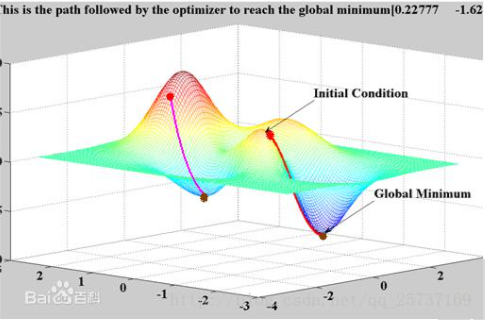
\includegraphics{./img/ch13/figure_13_15_1.png}
\caption{}
\end{figure}

图 13.8.1

\subsection{梯度消失/爆炸产生的原因?}\label{ux68afux5ea6ux6d88ux5931ux7206ux70b8ux4ea7ux751fux7684ux539fux56e0}

本质上,梯度消失和爆炸是一种情况。在深层网络中,由于网络过深,如果初始得到的梯度过小,或者传播途中在某一层上过小,则在之后的层上得到的梯度会越来越小,即产生了梯度消失。梯度爆炸也是同样的。一般地,不合理的初始化以及激活函数,如sigmoid等,都会导致梯度过大或者过小,从而引起消失/爆炸。

下面分别从网络深度角度以及激活函数角度进行解释:

(1)网络深度

若在网络很深时,若权重初始化较小,各层上的相乘得到的数值都会0-1之间的小数,而激活函数梯度也是0-1之间的数。那么连乘后,结果数值就会变得非常小,导致\textbf{梯度消失}。若权重初始化较大,大到乘以激活函数的导数都大于1,那么连乘后,可能会导致求导的结果很大,形成\textbf{梯度爆炸}。

(2)激活函数\\
如果激活函数选择不合适,比如使用
sigmoid,梯度消失就会很明显了,原因看下图,左图是sigmoid的函数图,右边是其导数的图像,如果使用sigmoid作为损失函数,其梯度是不可能超过0.25的,这样经过链式求导之后,很容易发生梯度消失。
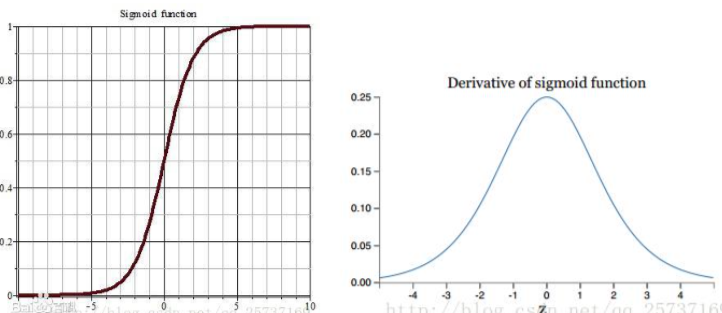
\includegraphics{./img/ch13/figure_13_15_2.png}

图 13.8.2 sigmod函数与其导数

\subsection{梯度消失、爆炸的解决方案}\label{ux68afux5ea6ux6d88ux5931ux7206ux70b8ux7684ux89e3ux51b3ux65b9ux6848}

\textbf{1、预训练加微调}\\
此方法来自Hinton在2006年发表的一篇论文,Hinton为了解决梯度的问题,提出采取无监督逐层训练方法,其基本思想是每次训练一层隐节点,训练时将上一层隐节点的输出作为输入,而本层隐节点的输出作为下一层隐节点的输入,此过程就是逐层``预训练''(pre-training);在预训练完成后,再对整个网络进行``微调''(fine-tunning)。Hinton在训练深度信念网络(Deep
Belief
Networks中,使用了这个方法,在各层预训练完成后,再利用BP算法对整个网络进行训练。此思想相当于是先寻找局部最优,然后整合起来寻找全局最优,此方法有一定的好处,但是目前应用的不是很多了。

\textbf{2、梯度剪切、正则}\\
梯度剪切这个方案主要是针对梯度爆炸提出的,其思想是设置一个梯度剪切阈值,然后更新梯度的时候,如果梯度超过这个阈值,那么就将其强制限制在这个范围之内。这可以防止梯度爆炸。\\
另外一种解决梯度爆炸的手段是采用权重正则化(weithts
regularization)比较常见的是L1和L2正则。

\textbf{3、ReLu、leakReLu等激活函数}\\
(1)ReLu:其函数的导数在正数部分是恒等于1,这样在深层网络中,在激活函数部分就不存在导致梯度过大或者过小的问题,缓解了梯度消失或者爆炸。同时也方便计算。当然,其也存在存在一些缺点,例如过滤到了负数部分,导致部分信息的丢失,输出的数据分布不在以0为中心,改变了数据分布。\\
(2)leakrelu:就是为了解决relu的0区间带来的影响,其数学表达为:leakrelu=max(k*x,0)其中k是leak系数,一般选择0.01或者0.02,或者通过学习而来。

\textbf{4、batchnorm}\\
Batchnorm是深度学习发展以来提出的最重要的成果之一了,目前已经被广泛的应用到了各大网络中,具有加速网络收敛速度,提升训练稳定性的效果,Batchnorm本质上是解决反向传播过程中的梯度问题。Batchnorm全名是Batch
Normalization,简称BN,即批规范化,通过规范化操作将输出信号x规范化到均值为0,方差为1保证网络的稳定性。

\textbf{5、残差结构}\\
残差的方式,能使得深层的网络梯度通过跳级连接路径直接返回到浅层部分,使得网络无论多深都能将梯度进行有效的回传。

\textbf{6、LSTM}\\
LSTM全称是长短期记忆网络(long-short term memory
networks),是不那么容易发生梯度消失的,主要原因在于LSTM内部复杂的``门''(gates)。在计算时,将过程中的梯度进行了抵消。

\section{深度学习为什么不用二阶优化?}\label{ux6df1ux5ea6ux5b66ux4e60ux4e3aux4ec0ux4e48ux4e0dux7528ux4e8cux9636ux4f18ux5316}

目前深度学习中,反向传播主要是依靠一阶梯度。二阶梯度在理论和实际上都是可以应用都网络中的,但相比于一阶梯度,二阶优化会存在以下一些主要问题:\\
(1)计算量大,训练非常慢。\\
(2)二阶方法能够更快地求得更高精度的解,这在浅层模型是有益的。而在神经网络这类深层模型中对参数的精度要求不高,甚至不高的精度对模型还有益处,能够提高模型的泛化能力。\\
(3)稳定性。二阶方法能更快求高精度的解,同样对数据本身要的精度也会相应的变高,这就会导致稳定性上的问题。

\section{为什么要设置单一数字评估指标,设置指标的意义?}\label{ux4e3aux4ec0ux4e48ux8981ux8bbeux7f6eux5355ux4e00ux6570ux5b57ux8bc4ux4f30ux6307ux6807ux8bbeux7f6eux6307ux6807ux7684ux610fux4e49}

在训练模型时,无论是调整超参数,还是调整不同的模型算法,我们都需要一个有效的评价指标,这个评价标准能帮助我们快速了解新的尝试后模型的性能是否更优。例如在分类时,我们通常会选择选择准确率,当样本不平衡时,查准率和查全率又会是更好的评价指标。所以在训练模型时,如果设置了单一数字的评估指标通常能很快的反应出我们模型的改进是否直接产生了收益,从而加速我们的算法改进过程。若在训练过程中,发现优化目标进一步深入,现有指标无法完全反应进一步的目标时,就需要重新选择评估指标了。

\section{训练/验证/测试集的定义及划分}\label{ux8badux7ec3ux9a8cux8bc1ux6d4bux8bd5ux96c6ux7684ux5b9aux4e49ux53caux5212ux5206}

训练、验证、测试集在机器学习领域是非常重要的三个内容。三者共同组成了整个项目的性能的上限和走向。

训练集:用于模型训练的样本集合,样本占用量是最大的;

验证集:用于训练过程中的模型性能评价,跟着性能评价才能更好的调参;

测试集:用于最终模型的一次最终评价,直接反应了模型的性能。

在划分上,可以分两种情况:

1、在样本量有限的情况下,有时候会把验证集和测试集合并。实际中,若划分为三类,那么训练集:验证集:测试集=6:2:2;若是两类,则训练集:验证集=7:3。这里需要主要在数据量不够多的情况,验证集和测试集需要占的数据比例比较多,以充分了解模型的泛化性。

2、在海量样本的情况下,这种情况在目前深度学习中会比较常见。此时由于数据量巨大,我们不需要将过多的数据用于验证和测试集。例如拥有1百万样本时,我们按训练集:验证集:测试集=98:1:1的比例划分,1\%的验证和1\%的测试集都已经拥有了1万个样本。这已足够验证模型性能了。

此外,三个数据集的划分不是一次就可以的,若调试过程中发现,三者得到的性能评价差异很大时,可以重新划分以确定是数据集划分的问题导致还是由模型本身导致的。其次,若评价指标发生变化,而导致模型性能差异在三者上很大时,同样可重新划分确认排除数据问题,以方便进一步的优化。

\section{什么是TOP5错误率?}\label{ux4ec0ux4e48ux662ftop5ux9519ux8befux7387}

通常对于分类系统而言,系统会对某个未知样本进行所有已知样本的匹配,并给出该未知样本在每个已知类别上的概率。其中最大的概率就是系统系统判定最可能的一个类别。TOP5则就是在前五个最大概率的类别。TOP5错误率,即预测最可能的五类都不是该样本类别的错误率。

TOP5错误率通常会用于在类别数量很多或者细粒度类别的模型系统。典型地,例如著名的ImageNet
,其包含了1000个类别。通常就会采用TOP5错误率。

\section{什么是泛化误差,如何理解方差和偏差?}\label{ux4ec0ux4e48ux662fux6cdbux5316ux8befux5deeux5982ux4f55ux7406ux89e3ux65b9ux5deeux548cux504fux5dee}

一般情况下,我们评价模型性能时都会使用泛化误差。泛化误差越低,模型性能越好。泛化误差可分解为方差、偏差和噪声三部分。这三部分中,噪声是个不可控因素,它的存在是算法一直无法解决的问题,很难约减,所以我们更多考虑的是方差和偏差。

方差和偏差在泛化误差上可做如下分解,假设我们的预测值为g(x),真实值为f(x),则均方误差为
\[
E((g(x)−f(x))2)
\]
这里假设不考虑噪声,g来代表预测值,f代表真实值,g¯=E(g)代表算法的期望预测,则有如下表达:
\[
\begin{align}
E(g-f)^2&=E(g^2-2gf+f^2)
\\&=E(g^2)-\bar g^2+(\bar g-f)^2
\\&=E(g^2)-2\bar g^2+\bar g^2+(\bar g-f)^2
\\&=E(g^2-2g\bar g^2+\bar g^2)+(\bar g-f)^2
\\&=\underbrace{E(g-\bar g)^2}_{var(x)}+\underbrace{(\bar g-f)^2}_{bias^2(x)}
\end{align}
\]
有上述公式可知,方差描述是理论期望和预测值之间的关系,这里的理论期望通常是指所有适用于模型的各种不同分布类型的数据集;偏差描述为真实值和预测值之间的关系,这里的真实值通常指某一个特定分布的数据集合。

所以综上方差表现为模型在各类分布数据的适应能力,方差越大,说明数据分布越分散,而偏差则表现为在特定分布上的适应能力,偏差越大越偏离真实值。

\section{如何提升模型的稳定性?}\label{ux5982ux4f55ux63d0ux5347ux6a21ux578bux7684ux7a33ux5b9aux6027}

评价模型不仅要从模型的主要指标上的性能,也要注重模型的稳定性。模型的稳定性体现在对不同样本之间的体现的差异。如模型的方差很大,那可以从如下几个方面进行考虑:

(1)正则化(L2, L1,
dropout):模型方差大,很可能来自于过拟合。正则化能有效的降低模型的复杂度,增加对更多分布的适应性。

(2)提前停止训练:提前停止是指模型在验证集上取得不错的性能时停止训练。这种方式本质和正则化是一个道理,能减少方差的同时增加的偏差。目的为了平衡训练集和未知数据之间在模型的表现差异。

(3)扩充训练集:正则化通过控制模型复杂度,来增加更多样本的适应性。那增加训练集让模型适应不同类型的数据本身就是一种最简单直接的方式提升模型稳定的方法,也是最可靠的一种方式。
与正则有所不同的是,扩充数据集既可以减小偏差又能减小方差。

(4)特征选择:过高的特征维度会使模型过拟合,减少特征维度和正则一样可能会处理好方差问题,但是同时会增大偏差。但需要注意的是若过度删减特征,很可能会删除很多有用的特征,降低模型的性能。所以需要多注意删减的特征对模型的性能的影响。

\section{有哪些改善模型的思路}\label{ux6709ux54eaux4e9bux6539ux5584ux6a21ux578bux7684ux601dux8def}

改善模型本质是如何优化模型,这本身是个很宽泛的问题。也是目前学界一直探索的目的,而从目前常规的手段上来说,一般可取如下几点。

\subsection{数据角度}\label{ux6570ux636eux89d2ux5ea6}

增强数据集。无论是有监督还是无监督学习,数据永远是最重要的驱动力。更多的类型数据对良好的模型能带来更好的稳定性和对未知数据的可预见性。对模型来说,``看到过的总比没看到的更具有判别的信心''。但增大数据并不是盲目的,模型容限能力不高的情况下即使增大数据也对模型毫无意义。而从数据获取的成本角度,对现有数据进行有效的扩充也是个非常有效且实际的方式。良好的数据处理,常见的处理方式如数据缩放、归一化和标准化等。

\subsection{ 模型角度}\label{ux6a21ux578bux89d2ux5ea6}

模型的容限能力决定着模型可优化的空间。在数据量充足的前提下,对同类型的模型,增大模型规模来提升容限无疑是最直接和有效的手段。但越大的参数模型优化也会越难,所以需要在合理的范围内对模型进行参数规模的修改。而不同类型的模型,在不同数据上的优化成本都可能不一样,所以在探索模型时需要尽可能挑选优化简单,训练效率更高的模型进行训练。

\subsection{调参优化角度}\label{ux8c03ux53c2ux4f18ux5316ux89d2ux5ea6}

如果你知道模型的性能为什么不再提高了,那已经向提升性能跨出了一大步。
超参数调整本身是一个比较大的问题。一般可以包含模型初始化的配置,优化算法的选取、学习率的策略以及如何配置正则和损失函数等等。这里需要提出的是对于同一优化算法,相近参数规模的前提下,不同类型的模型总能表现出不同的性能。这实际上就是模型优化成本。从这个角度的反方向来考虑,同一模型也总能找到一种比较适合的优化算法。所以确定了模型后选择一个适合模型的优化算法也是非常重要的手段。

\subsection{ 训练角度}\label{ux8badux7ec3ux89d2ux5ea6}

很多时候我们会把优化和训练放一起。但这里我们分开来讲,主要是为了强调充分的训练。在越大规模的数据集或者模型上,诚然一个好的优化算法总能加速收敛。但你在未探索到模型的上限之前,永远不知道训练多久算训练完成。所以在改善模型上充分训练永远是最必要的过程。充分训练的含义不仅仅只是增大训练轮数。有效的学习率衰减和正则同样是充分训练中非常必要的手段。

\section{如何快速构建有效初始模型?}\label{ux5982ux4f55ux5febux901fux6784ux5efaux6709ux6548ux521dux59cbux6a21ux578b}

​
构建一个有效的初始模型能帮助我们快速了解数据的质量和确定模型构建的方向。构建一个良好的初始模型,一般需要注意如下几点:

​
1、了解``对手''。这里的``对手''通常是指数据,我们在得到数据时,第一步是需要了解数据特点和使用场合。了解数据特点能帮助我们快速定位如何进行建模。确定使用场合能帮助我们进一步确定模型需要优化的方向。数据特点一般需要了解例如数据集规模、训练集和验证集是否匹配、样本的分布是否均匀、数据是否存在缺失值等等。

​
2、站在巨人肩膀上。根据数据特点,我们通常能匹配到一个现有比较优秀的模型。这类模型都通常能在类似数据上表现出一个比较不错的性能。

​
3、一切从简。初始模型的作用在于迅速了解数据质量和特点,所以模型的性能通常不需要达到很高,模型复杂度也不需要很高。例如,做图像分类时,我们在使用预训练模型时,不需要一开始就使用例如ResNet152这类模型巨大,复杂度过高的模型。这在数据量较小时,很容易造成过拟合而导致出现我们对数据产生一些误导性的判断,此外也增加了额外训练构建时间。所以使用更小更简单的模型以及损失函数来试探数据是相比更明智的选择。

​
4、总比瞎猜强。构建模型的意义在于建立一个高效的模型,虽然初始模型我们不对性能做过高的要求。但前提在于必须要比随机猜测好,不然构建模型的意义就不存在了。

​
5、解剖模型。一旦确定了一个初始模型时,无论你对该模型多熟悉,当其面对一批新数据时,你永远需要重新去认识这个模型,因为你永远不确定模型内部到底发生了些什么。解剖模型一般需要在训练时注意误差变化、注意训练和验证集的差异;出现一些NAN或者INf等情况时,需要打印观察内部输出,确定问题出现的时间和位置;在完成训练后,需要测试模型的输出是否正确合理,以确认评价指标是否符合该数据场景。无论使用任何一种模型,我们都不能把它当做黑盒去看待。

\section{如何通过模型重新观察数据?}\label{ux5982ux4f55ux901aux8fc7ux6a21ux578bux91cdux65b0ux89c2ux5bdfux6570ux636e}

​
对于这个问题,与其说如何做,倒不如说这个问题是用来强调这样做的重要性。如何重新观察数据其实不难,而是很多读者,会忽略这一项过程的重要性。

​
通过模型重新观察数据,不仅能让我们了解模型情况,也能让我们对数据质量产生进一步的理解。目前深度学习在监督学习领域成就是非常显著的。监督学习需要依赖大量的人为标注,人为标注很难确定是否使用的数据中是否存在错误标注或者漏标注等问题。这无论是哪种情况都会影响我们对模型的判断。所以通过模型重新验证数据质量是非常重要的一步。很多初学者,通常会忽略这一点,而导致出现对模型的一些误判,严重时甚至会影响整个建模方向。此外,对于若出现一些过拟合的情况,我们也可以通过观察来了解模型。例如分类任务,样本严重不平衡时,模型全预测到了一边时,其正确率仍然很高,但显然模型已经出现了问题。

\section{如何解决数据不匹配问题?}\label{ux5982ux4f55ux89e3ux51b3ux6570ux636eux4e0dux5339ux914dux95eeux9898}

\subsection{如何定位数据不匹配?}\label{ux5982ux4f55ux5b9aux4f4dux6570ux636eux4e0dux5339ux914d}

​
数据不匹配问题是个不容易定位和解决的问题。这个问题出现总会和模型过拟合表现很相似,即在训练集上能体现非常不错的性能,但在测试集上表现总是差强人意但区别在于如果遇到是数据不匹配的问题,通常在用一批和训
练集有看相同或者相似分布的数据上仍然能取得不错的结果。但很多时候,当测试集上结果表现很差时,很多初学
者可能会直接将问题定位在模型过拟合上,最后对模型尝试各种方法后,性能却始终不能得到有效提升。当遇到这
种情况时,建议先定位出是否存在数据不匹配的问题。最简单的验证方式就是可以从训练集中挑选出一部分数据作
为验证集,重新划分后训练和验证模型表现。

\subsection{举例常见几个数据不匹配的场景?}\label{ux4e3eux4f8bux5e38ux89c1ux51e0ux4e2aux6570ux636eux4e0dux5339ux914dux7684ux573aux666f}

​
例如设计款识别物体的app时,实际场景的图片均来自于手机拍摄,而训练集确是来自于网上各类抓取下来的图
片。例如在图像去噪、去模糊、去雾、超分辨率等图像处理场景时,由于大量数据的难以获取,因此都会采用人为
假设合成的图像进行训练,这时候应用到实际场景中也容易出现不匹配的问题

\subsection{如何解决数据不匹配问题?}\label{ux5982ux4f55ux89e3ux51b3ux6570ux636eux4e0dux5339ux914dux95eeux9898-1}

​ 数据不匹配是个很难有固定方法来解决的问题。这里提供几条供参考的途径: ​
1、收集更多符合实际场最需要的数据。这似乎是最简单但也最难方式 ​
2、对结果做错误分析。找出数据集中出错的数据和正确数据之间的特点和区别,这对你无论是进行后续模型的分析或者是数据的处理提供非常有效的思路。注意,这里的数据集包括训练集和测试集
​
3、数据集增强。数据集增强并不意味看数据集越大越好,其目的是丰富数据的分布以适应更多的变化当遇到数
据不匹配时,对数据处理般可以有两种方式。其一,合成或处理更多接近需要的数据特点。其二,对所有数据包
括实际场景数据都进行处理,将所有数据都统一到另一个分布上,统一出一种新的特点。

\subsection{如何提高深度学习系统的性能}\label{ux5982ux4f55ux63d0ux9ad8ux6df1ux5ea6ux5b66ux4e60ux7cfbux7edfux7684ux6027ux80fd}

​ 当我们要试图提高深度学习系统的性能时,目前我们大致可以从三方面考虑:

​
1、提高模型的结构,比如增加神经网络的层数,或者将简单的神经元单位换成复杂的
LSTM 神经元,比如在自然语言处理领域内,利用 LSTM
模型挖掘语法分析的优势。

​
2、改进模型的初始化方式,保证早期梯度具有某些有益的性质,或者具备大量的稀疏性,或者利用线性代数原理的优势。

​
3、选择更强大的学习算法,比如对度梯度更新的方式,也可以是采用除以先前梯度
L2 范数来更新所有参数,甚至还可以选用计算代价较大的二阶算法。

% \section{参考文献}\label{ux53c2ux8003ux6587ux732e}

% {[}1{]} 冯宇旭, 李裕梅. 深度学习优化器方法及学习率衰减方式综述{[}J{]}.
% 数据挖掘, 2018, 8(4): 186-200.
